\documentclass[10pt, conference, letterpaper]{IEEEtran}

\usepackage{algorithm}
\usepackage{algorithmicx}
\usepackage{algpseudocode}
\usepackage{amsfonts}
\usepackage{amsmath}
\usepackage{amssymb}
\usepackage[ansinew]{inputenc} 
\usepackage{xcolor}
\usepackage{mathtools}
\usepackage{graphicx}
\usepackage{caption}
\usepackage{subcaption}
\usepackage{import}
\usepackage{multirow}
\usepackage{cite}
\usepackage[export]{adjustbox}
\usepackage{breqn}
\usepackage{mathrsfs}
\usepackage{acronym}
%\usepackage[keeplastbox]{flushend}
\usepackage{setspace}
\usepackage{bm}
\usepackage{stackengine}
\usepackage{hyperref}
\usepackage{listings}
\usepackage{booktabs}

\lstset{%
 backgroundcolor=\color[gray]{.85},
 basicstyle=\small\ttfamily,
 breaklines = true,
 keywordstyle=\color{red!75},
 columns=fullflexible,
}%

\lstdefinelanguage{BibTeX}
  {keywords={%
      @article,@book,@collectedbook,@conference,@electronic,@ieeetranbstctl,%
      @inbook,@incollectedbook,@incollection,@injournal,@inproceedings,%
      @manual,@mastersthesis,@misc,@patent,@periodical,@phdthesis,@preamble,%
      @proceedings,@standard,@string,@techreport,@unpublished%
      },
   comment=[l][\itshape]{@comment},
   sensitive=false,
  }

\usepackage{listings}

% listings settings from classicthesis package by
% Andr\'{e} Miede
\lstset{language=[LaTeX]Tex,%C++,
    keywordstyle=\color{RoyalBlue},%\bfseries,
    basicstyle=\small\ttfamily,
    %identifierstyle=\color{NavyBlue},
    commentstyle=\color{Green}\ttfamily,
    stringstyle=\rmfamily,
    numbers=none,%left,%
    numberstyle=\scriptsize,%\tiny
    stepnumber=5,
    numbersep=8pt,
    showstringspaces=false,
    breaklines=true,
    frameround=ftff,
    frame=single
    %frame=L
}

\renewcommand{\thetable}{\arabic{table}}
\renewcommand{\thesubtable}{\alph{subtable}}

\DeclareMathOperator*{\argmin}{arg\,min}
\DeclareMathOperator*{\argmax}{arg\,max}

\def\delequal{\mathrel{\ensurestackMath{\stackon[1pt]{=}{\scriptscriptstyle\Delta}}}}

\graphicspath{{./figures/}}
\setlength{\belowcaptionskip}{0mm}
\setlength{\textfloatsep}{8pt}

\newcommand{\eq}[1]{Eq.~\eqref{#1}}
\newcommand{\fig}[1]{Fig.~\ref{#1}}
\newcommand{\tab}[1]{Tab.~\ref{#1}}
\newcommand{\secref}[1]{Section~\ref{#1}}

\newcommand\MR[1]{\textcolor{blue}{#1}}
\newcommand\red[1]{\textcolor{red}{#1}}
\newcommand{\mytexttilde}{{\raise.17ex\hbox{$\scriptstyle\mathtt{\sim}$}}}

%\renewcommand{\baselinestretch}{0.98}
% \renewcommand{\bottomfraction}{0.8}
% \setlength{\abovecaptionskip}{0pt}
\setlength{\columnsep}{0.2in}

% \IEEEoverridecommandlockouts\IEEEpubid{\makebox[\columnwidth]{PUT COPYRIGHT NOTICE HERE \hfill} \hspace{\columnsep}\makebox[\columnwidth]{ }} 

\title{``Analysis and comparison of the main techniques \\ designed for Environmental Sound Classification''}

\author{Mattia Pujatti $^\dag$
\thanks{$^\dag$ Physics of Data, Department of Physics and Astronomy, University of Padova, email: mattia.pujatti.1@studenti.unipd.it}
} 

\IEEEoverridecommandlockouts

\newcounter{remark}[section]
\newenvironment{remark}[1][]{\refstepcounter{remark}\par\medskip
   \textbf{Remark~\thesection.\theremark. #1} \rmfamily}{\medskip}

\begin{document}

\maketitle

\begin{abstract}
Future vehicular communication networks call for new solutions to support their capacity demands, by leveraging the potential of the \mbox{millimeter-wave} (\mbox{mm-wave}) spectrum. Mobility, in particular, poses severe challenges in their design, and as such shall be accounted for. A key question in \mbox{mm-wave} vehicular networks is how to optimize the \mbox{trade-off} between directive Data Transmission (DT) and directional Beam Training (BT), which enables it. In this paper, learning tools are investigated to optimize this \mbox{trade-off}. In the proposed scenario, a Base Station (BS) uses BT to establish a \mbox{mm-wave} directive link towards a Mobile User (MU) moving along a road. To control the BT/DT \mbox{trade-off}, a Partially Observable (PO) Markov Decision Process (MDP) is formulated, where the system state corresponds to the position of the MU within the road link. The goal is to maximize the number of bits delivered by the BS to the MU over the communication session, under a power constraint. The resulting optimal policies reveal that adaptive BT/DT procedures significantly outperform \mbox{common-sense} heuristic schemes, and that specific mobility features, such as user position estimates, can be effectively used to enhance the overall system performance and optimize the available system resources.\\ 

\end{abstract}

\IEEEkeywords
Supervised Learning, Neural Networks, Audio Classification, Nested Cross Validation, Sound Features.
\endIEEEkeywords


\input{Intro}

% !TEX root = report.tex

\section{Related Work}
\label{sec:related_work}

In recent years, audio recognition systems have gained so much popularity in the machine learning world, mainly because of the developments in the artificial intelligence field. However, the research has focused mostly on speech recognition tasks, music classification and acoustic scene classification, while identification of environmental sounds was took less in consideration. One of the main reasons for this, as anticipated, was the scarcity of suitable and publicly available datasets. But when, in 2015, K. Piczak realized and made public a collection of 2000 environmental short sound clips, under the name of ESC-50 dataset \cite{piczak2015dataset}, people's interest started rising again, together with a sort of "competition", in which many classification methods were applied in order to obtain the higher accuracy over it. In the github page of the author \cite{piczakgithub} there is, in fact, a table summarizing more than 30 papers written on top of ESC-50, each of them proposing a different approach to classify those sounds. Piczak itself, in its first papers \cite{piczak2015dataset}, suggested the usage of a few "canonical" machine learning classifiers (mostly based on features extraction), and compared the results with the ones obtained from a set of human participants. Moreover, in a second paper \cite{piczak_cnn}, proposed instead the employment of convolutional neural networks, to be applied over the spectrograms derived from the clips: apparently, this approach outperformed the baseline implementation and, in fact, defined the new state of the art for environmental sound classification.\\
In the table mentioned earlier, collecting all the recent developments for this specific task and exploiting ESC-50, several different approaches are proposed: many of them are based on speech recognition-like models (MFCC coefficients, \cite{piczak2015dataset, freitag2017}), while many others are improved version of the CNN implementations (different representations, architectures, preprocessing phases \cite{Huzaifah17, soundnet, boddapati2017, aclnet, ensemble_stacked_cnn}). The head of the ranking is entirely covered by the second type of technique, that apparently outperforms the first one from any point of view. Also, many of the methods listed, rely on pretrained models, ad-hoc data augmentation and very complex architectures, mostly realized combining different machine learning prototypes. Actually, only a few approaches, all based on CNNs, are able to overcome the human classification accuracy ($81.30\%$) over ESC-50, with the best model reaching even the $94\%$ of correctly classified samples. Features extraction models, instead, appear much less frequently in the table (people started losing interest versus them) and they can all be found under the humans' accuracy threshold (the best result, $64.30\%$, was achieved exploiting the combination of a RNN autoencoder and a Multi-Layer Perceptron \cite{freitag2017}).

% !TEX root = template.tex

\section{Processing Pipeline}
\label{sec:processing_architecture}

\begin{remark}
\textbf{On tailoring the paper structure to your needs:} The structure recommended for the previous sections is rather standard and could work for different papers with differing technical content, the structure and the paper content from here on highly depends on the type of paper, possibilities are: mostly based on theoretical analysis, showing experimental design/activity, proposing a new technique and analyzing its performance via experiments or simulation. For the HDA course we deal with machine learning and, in detail, with training and testing neural network architectures to perform some specific inference or classification task. The following structure and comments are specifically addressing this type of technical content.
\end{remark}

\begin{remark}
\textbf{Why having this section:} With this section, we start the technical description with a {\it high level} introduction of your work (e.g., processing pipeline). Here, you do not have to necessarily go into the technical details of every block/algorithm of your design, this will be done later as the paper develops. What I would like to see here is a high level description of the approach, i.e., which processing blocks you used, what they do (in words) and how these were combined, etc. This section should introduce the reader to your design, explain the different parts/blocks, how they interact and why. You should not delve into technical details for each block, but you should rather explain the big picture. \MR{Besides a well written explanation, I often use a nice diagram containing the various blocks and detailing their interrelations.}
\end{remark} 

\noindent \textbf{Writing tips:} Sections, Figures and Tables are usually shortened as Sec., Fig., Tab. 
\begin{itemize}
\item \textbf{Cross referencing:} In Latex, cross referencing is easy. You need to label an object through the \texttt{\textbackslash label\{labelid\}} command and referencing it where you need it through the \texttt{\textbackslash ref\{labelid\}} command. 
\item \textbf{Suggestion:} I suggest to cross reference a table using \texttt{Tab.\mytexttilde\textbackslash ref\{tab:tableid\}}, the same holds for figures and sections, by just replacing ``\texttt{Tab.}'' with ``\texttt{Fig.}'' and ``\texttt{Sec.}''. Of course when defining the table, you need to add a Latex command \texttt{\textbackslash label\{tab:tableid\}} in the right place inside the table Latex environment to \mbox{cross-link} it. The tag \texttt{tab:tableid} is user defined and is the identifier that you associate with the table in question. You could call it \texttt{pippo} of you wish, but I recommend to use something like ``\texttt{tab:tableid}'' for tables, ``\texttt{eq:eqid}'' for equations, ``\texttt{sec:secid}'' for sections and so forth, where \texttt{tableid} has to be unique for each table in the document. The same applies to figures and all other objects. I guess you got the idea. This will lead to a neat Latex code and will facilitate cross referencing while avoiding duplicate labels, especially in large Latex documents (think of a book for example). 
\item \textbf{But what about the tilde?} This is a nice trick I have learned from a friend (many years ago from Prof. Frank Fitzek, now at TU Dresden). When you write \texttt{Tab.\mytexttilde\textbackslash ref\{tab:tableid\}} Latex knows that \texttt{Tab.} and the corresponding table number \texttt{\textbackslash ref\{tab:tableid\}} must be displayed within the same line, i.e., they can never be broken across lines. This is nice and desirable I believe. I always use it for all referenced material, including citations; example: ``As done in\texttt{\mytexttilde\textbackslash cite\{suppa-wu-2019\}}.''
\item \textbf{More about breaking stuff across lines} often times you have composed words, in line equations, etc. and for some reason you would like Latex to never break them across lines. Example: the Latex command \texttt{\textbackslash mbox\{Neural Networks (NN)\}} is processed by Latex so that ``\mbox{Neural Networks (NN)}'' is never broken across lines. I use this very often, also for inline equations that I do not want Latex to split across subsequent lines.
\end{itemize}

\section{Signals and Features}
\label{sec:model}

Being a machine learning paper, I would have here a section describing the signals you have been working on. If possible, you should describe, in order, 
\begin{enumerate}
\item the measurement setup (if relevant), how input data is formatted (e.g., vectors of fixed size measured at regular sampling times), 
\item how the signals were \mbox{pre-processed}, e.g., to remove noise, artifacts, fill gaps (missing points) or to re-interpolate the signals to represent them through a constant sampling rate, etc.
\item after this, you should describe how {\it feature vectors} were obtained from the \mbox{pre-processed} signals. If signals are {\it time series} this also implies stating the segmentation / windowing strategy that you adopted, to then describe how you obtained a feature vector for each time window. Also, if you use existing feature extraction approaches, you may want to briefly describe them as well, in addition to (and before) your own (possibly new) feature extraction method.
\end{enumerate}

\MR{Last but not least, this section should also contain information on how you have split the dataset into training, validation and test sets. This will be briefly recalled within the ``Results'' section.}

\section{Learning Framework}
\label{sec:learning_framework}

Here you finally describe the learning strategy / algorithm that you conceived and used to solve the problem at stake. A good diagram to exemplify how learning is carried out is often very useful. In this section, you should describe the learning model, its parameters, any optimization over a given parameter set, etc. You can organize this section into \mbox{sub-sections}. You are free to choose the most appropriate structure.

\begin{remark}
Note that the diagram that you put here differs from that of Section~\ref{sec:processing_architecture} as here you show the details of how your learning framework, or the core of it, is built. In Section~\ref{sec:processing_architecture} you instead provide a high-level description of the involved processing blocks, i.e., you describe the {\it processing flow} and the rationale behind it.
\end{remark}

\noindent \textbf{On math typesetting:} there are many Latex tricks that you should use to produce a high quality technical essay. A few are listed below, in random order:
\begin{itemize}
\item \textbf{Vectors and matrices:} $x$ is a scalar, whereas $\bm{x}$ (in bold) is a vector, and $\bm{X}$ is a matrix with elements $\bm{X} = [x_{ij}]$. For bold symbols you may use the \texttt{\textbackslash bm} Latex command, e.g., \texttt{\textbackslash bm(x)}.
\item \textbf{Operators:} such as $\max$, $\min$, $\arg\!\max$, $\arg\!\min$ and special functions such as $\log(\cdot)$, $\exp(\cdot)$, $\sin(\cdot)$, $\cos(\cdot)$ are obtained through specific latex commands \texttt{\textbackslash min}, \texttt{\textbackslash max}, \texttt{\textbackslash arg\textbackslash!min}, \texttt{\textbackslash arg\textbackslash!max}, \texttt{\textbackslash log}, \texttt{\textbackslash exp}, \texttt{\textbackslash sin}, \texttt{\textbackslash cos}, etc. Use them! $log$, $exp$, $min$, $sin$, $cos$, etc., look ugly.
\item \textbf{Sets} can be represented through calligraphic fonts, e.g., $\mathcal{S}$, $\mathcal{F}$, $\mathcal{B}$, etc., obtained using the Latex command \texttt{\textbackslash mathcal{\{S\}}}, etc.
\item \textbf{Equations:} for a single equation use the \texttt{equation} Latex environment. Example: 
\begin{equation}
\label{eq:sigmoid}
\sigma(x) = \frac{1}{1+e^{-x}}.
\end{equation} 
Now, using round brackets $($ and $)$ we get
\begin{equation}
\label{eq:sigmoid_comma}
\sigma(x) = (\frac{1}{1+e^{-x}}),
\end{equation} 
but this looks ugly, you should use ``\texttt{\textbackslash left (}'' for ``$($'' and ``\texttt{\textbackslash right )}'' for ``$)$'', obtaining
\begin{equation}
\sigma(x) = \left ( \frac{1}{1+e^{-x}} \right ).
\end{equation} 
\item \textbf{Punctuation:} Displayed equations are usually considered to be part of the text and, in turn, they will get the very same punctuation as if they were inline with the text (and part of the sentence). If the sentence ends with a displayed equation, the equation gets a period ``.'' right after it, see Eq.~(\ref{eq:sigmoid}). iI the equation is instead part of a running sentence, which is continued after it, then the equation may be ended by a ``,'' as in Eq.~(\ref{eq:sigmoid_comma}). Use the standard grammar rules and your good sense of flow to assess how equations should be punctuated, I usually read through as if they were plain text.
\end{itemize} 



\input{results}

% !TEX root = report.tex

\section{Concluding Remarks}
\label{sec:conclusions}

The goal of this project was to study and implement the main approaches developed so far in the field of environmental sound classification, especially considering the limited nature of dataset available for our purposes. So, given the ESC-50 dataset, we have presented the main techniques designed and implemented with the objective of classifying those clips. Even if we didn't managed to reach the very high accuracies of several professional works, we can be quite satisfied of several results obtained and summarized in the last paragraph of the previous section.\\
Further improvements could be simply deepening one of the models analyzed, maybe trying with more complex architectures, different preprocessing steps or even testing pre-trained models. However, actually the biggest problem is the absence of large datasets, since 2000 clips is not enough to construct a credible statistics for generic applications, even exploiting nested cross validation. \\
In any case, the strong interest of the scientific community in speech recognition tasks, and the consequent improvements in sound classification, will for sure benefit also the branch of environmental sounds. \\
Regarding myself, instead, I can say that I practiced a lot with several Python libraries dedicated to machine learning (\textit{SKLearn, Keras, Tensorflow}), especially for what involves data management and preprocessing. Moreover, this was my first project exploiting sound data, and so I learned a lot about audio features and track manipulation.\\  
The most challenging part of this project was, for sure, determining a way to speed up the training processes (that could take up to many hours for each model), keeping, at the same time, a low memory usage, and ending up with a reliable statistics for the results. 






\nocite{*}
\bibliography{biblio}
\bibliographystyle{ieeetr}

\newpage
\appendix

% !TEX root = report.tex

\subsection{Correlation matrix}
\label{app:correlation_matrix}
In the large figure \ref{fig:correlation_matrix} is represented the correlation matrix among the 55 different high-level audio features (or, better, distributions) that have been extracted from each clip of ESC-50, according to the procedure explained in section \ref{sec:features_extraction}.\\
Analyzing this correlation matrix we can make several interesting observations about the information that has been effectively extracted from the audio samples:
\begin{itemize}
	\itemsep0em
	\item as expected, variables that are already "grouped", like MFCCs, chroma features, etc. manifest some kind of dependence among each other (especially the variables in the chromagram that appear to be strongly correlated);
	\item spectral features and zero-crossing rate, even if computed separately, as "single" features, exhibit some correlations; the reason is that they simply all come from the analysis of the same spectrogram;
	\item spectral features and MFCCs seems somehow anti-correlated;
	\item energy and corresponding derivatives are less likely to reveal any kind of dependence with any other variable;
	\item an interesting correlation appears between the MFCCs and the chroma features;
	\item just to precise, many of the anti-correlations involving the deltas that can be evinced from the plot are originated simply by the fact that such features are directly calculated from the others and so the dependence is obvious.
\end{itemize}

So, to conclude, many of the features extracted exhibit some kind of correlations/anti-correlations among each other, and for this reason they probably share part of the information carried. Further proof of this conclusion can be found in appendix \ref{app:dim_reduction}, when talking about Principal Component Analysis.

\begin{figure*}[t]
	\centering
	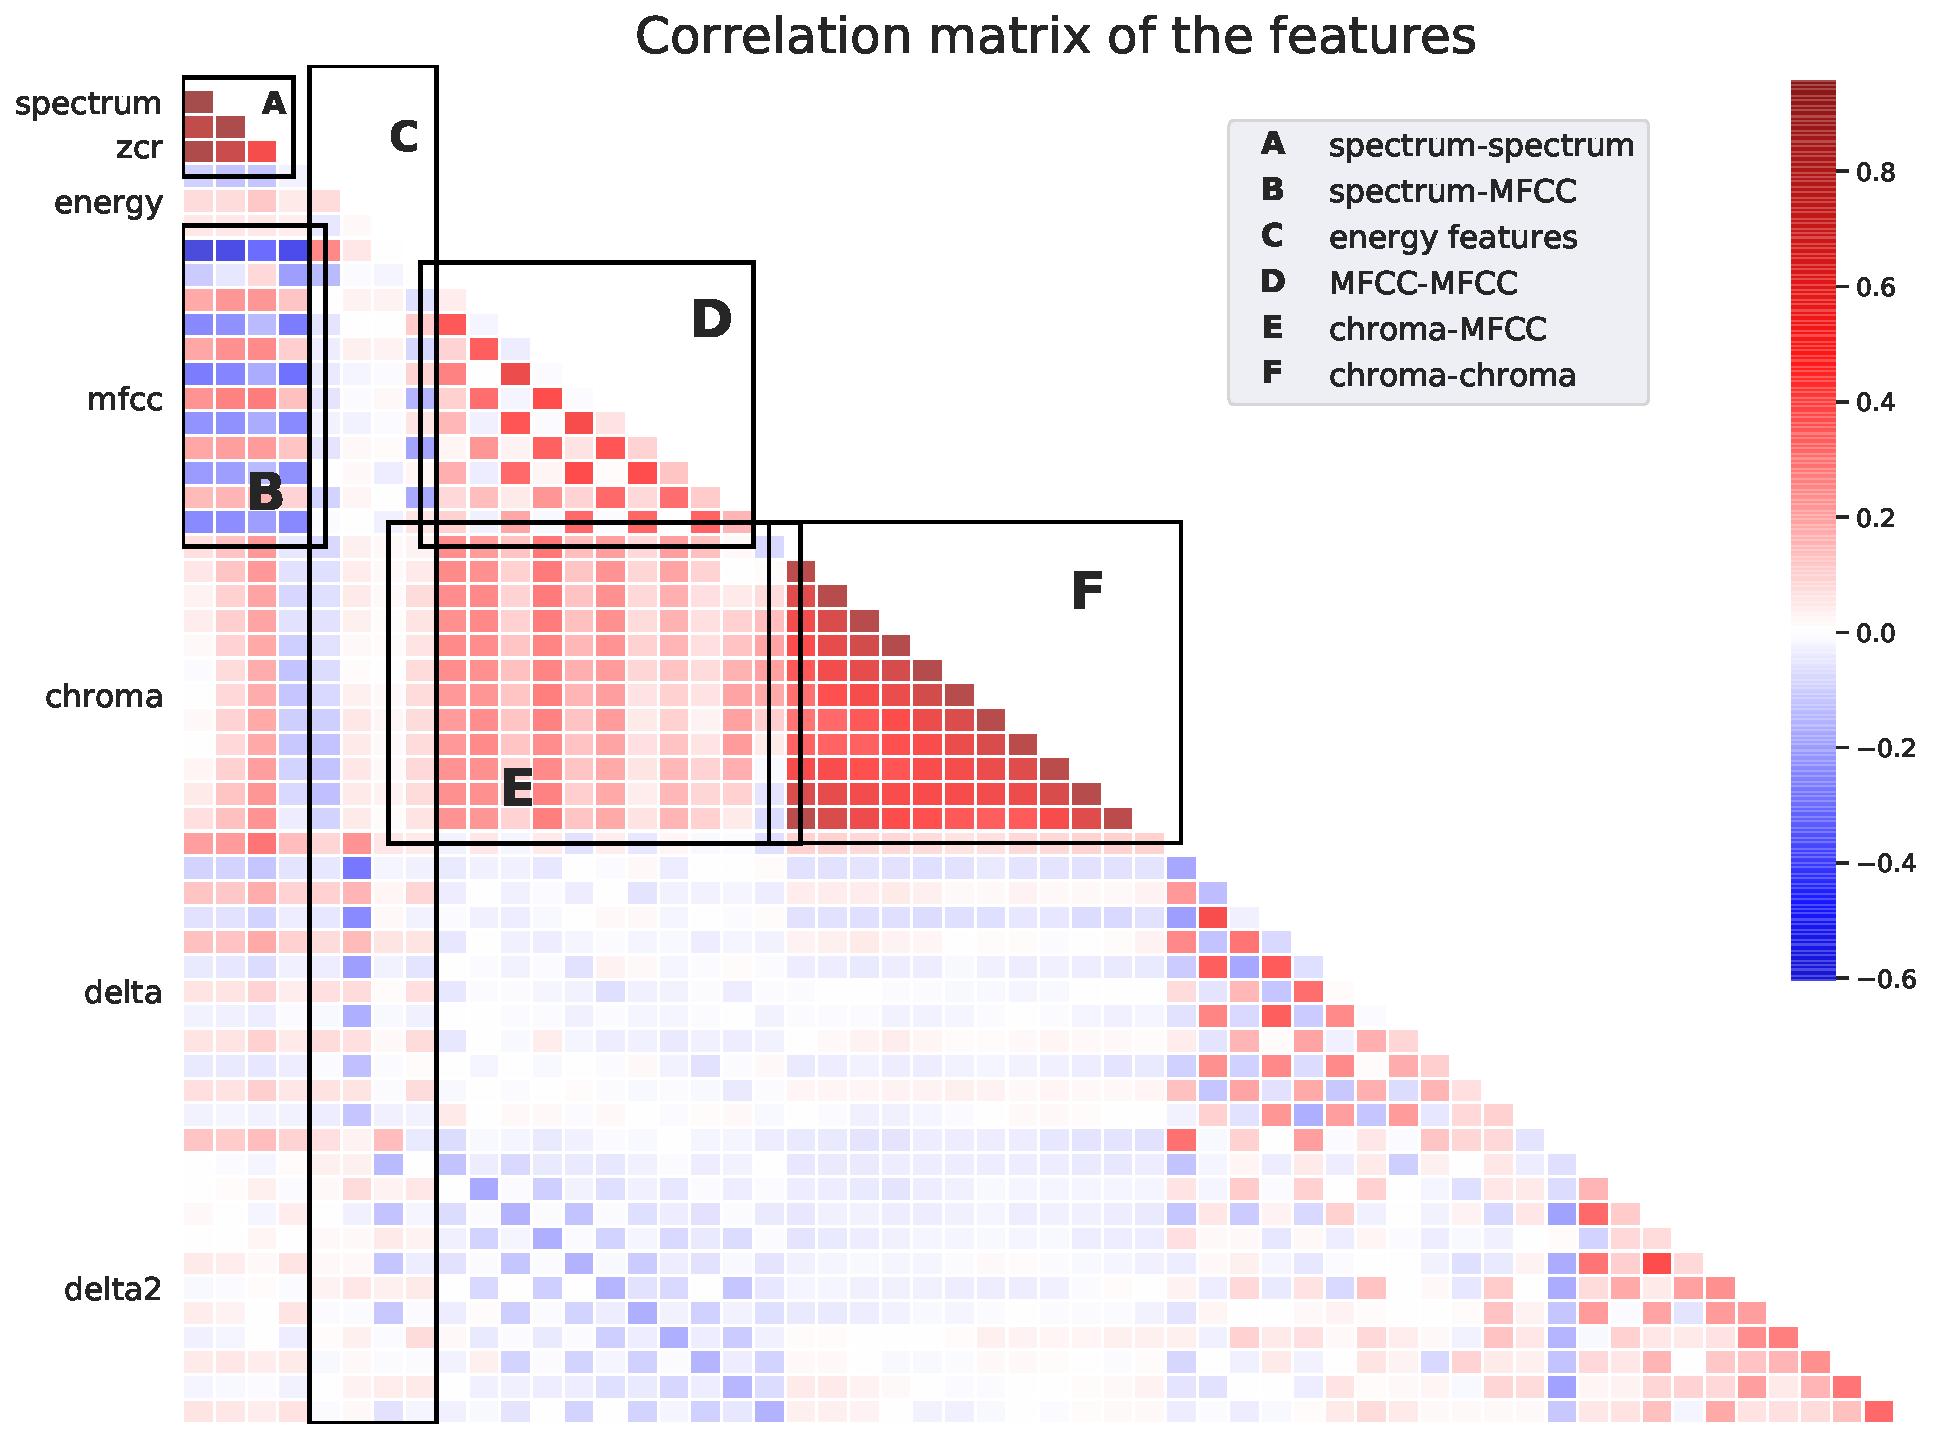
\includegraphics[scale=0.5]{pictures/correlation_matrix}
	\caption{Correlation matrix of the 55 high-level audio features extracted to represent the clips contained in ESC-50, as explained in section \ref{sec:features_extraction}.}
	\label{fig:correlation_matrix}
\end{figure*}
% !TEX root = report.tex

\subsection{Nested Cross Validation}
\label{app:nested_CV}

A non-nested approach consists in using the same cross-validation procedure and data both to tune and select a model, but this is likely to lead to an optimistically biased evaluation of the model performance (because of information leakage). Nested Cross-Validation (Nested-CV) nests cross-validation and hyperparameter tuning exploiting two different KFold (or stratified KFold) splitting, such that in the inner loop the score is approximately maximized by fitting a model to each training set, and then directly maximized in selecting (hyper)parameters over the validation set; in the outer loop, instead, the generalization error is estimated by averaging test set scores over several dataset splits. Under this procedure, hyperparameter search does not have the opportunity of overfitting the dataset as it is only exposed to a subset of it, provided by the outer cross-validation. This reduces, if not eliminates, the risk overfitting and should provide a less biased estimate of a tuned model's performance on the dataset. Obviously, this does not come without any additional cost, since you dramatically increase the number of intermediate steps: if $n*k$ models are fit and evaluated as part of a traditional non-nested CV for a given model, then this number is increased to $k*n*k$ as the procedure is then performed k more times for each fold in the outer loop of nested CV.

\subsection{Results of the GridSearch}
\label{app:featclass_best_params}

In this section we leave a brief recap of the combinations of hyperparameters, that we have found thanks to a nested cross validation applied to ESC-50, to guarantee the highest level in term of accuracy over the dataset.

\begin{table}[!ht]
	\centering
	\begin{tabular}{p{0.2\textwidth} p{0.2\textwidth}}
		\toprule
		\textbf{Model} & \textbf{Best hyperparameters} \\
		\midrule
		Random Forest & \begin{itemize} 
			\item \textit{bootstrap}: True;
			\item \textit{max\_depth}: 15;
			\item \textit{n\_estimators}: 500.
		\end{itemize} \\
		\midrule
		Multi-Layer Perceptron & \begin{itemize}
			\item \textit{activation}: relu;
			\item \textit{hidden\_layer\_sizes}: 512;
			\item \textit{learning\_rate\_init}: 0.01;
			\item \textit{solver}: adam.
		\end{itemize} \\
		\midrule
		K-Neighbors Classifier  & \begin{itemize}
			\item \textit{algorithm}: auto;
			\item \textit{leaf\_size}: 10;
			\item \textit{n\_neighbors}: 2;
			\item \textit{weigths}: distance;
		\end{itemize} \\
		\midrule
		Support Vector Machine  & \begin{itemize}
			\item \textit{C}: 0.1;
			\item \textit{kernel}: linear.
		\end{itemize} \\
		\midrule
		Feed-Forward Network & \begin{itemize}
			\item \textit{batch\_size}: 128;
			\item \textit{epochs}: 150;
			\item \textit{lr}: 0.001;
			\item \textit{optimizer}: adamax.
		\end{itemize} \\	
		\bottomrule
	\end{tabular}
	\caption{Summary of the best combinations of hyperparameters for the features classifiers, found thanks to a nested CV.}
	\label{tab:summay_best_params}
\end{table}
% !TEX root = report.tex

\subsection{Further Analysis}
\label{app:further_analysis}

\subsubsection{Impact of the dimensionality reduction}
\label{app:dim_reduction}
Working with large sized vectors of features can be very memory and time demanding, especially when training a complex classifier, maybe with a large number of parameters. For this reason one usually implement, before passing the data to the algorithm, a dimensionality reduction step, that in this case is a \textit{Principal Component Analysis}, with the purpose of reducing the dimension of each input vector, while keeping the "information" provided by it as untouched as possible. But how much this step will influence the performances of the classifiers? Let's first give a look at figure \ref{fig:cev}, that allows to determine the number of principal components to keep without losing too much of that "information". Basically, during the PCA, you are projecting your data into a smaller dimensional vector space, and each principal component corresponds to an eigenvalue of the covariance matrix of the dataset: reducing the size of the problem means keeping only the first $K$ eigenvalues, i.e. the ones with the higher variance. In the plot it is represented the \textit{cumulative explained variance} as a function of the number of components kept: the closer to 1 is the value, the more will be the information represented.
\begin{figure}[!h]
	\centering
	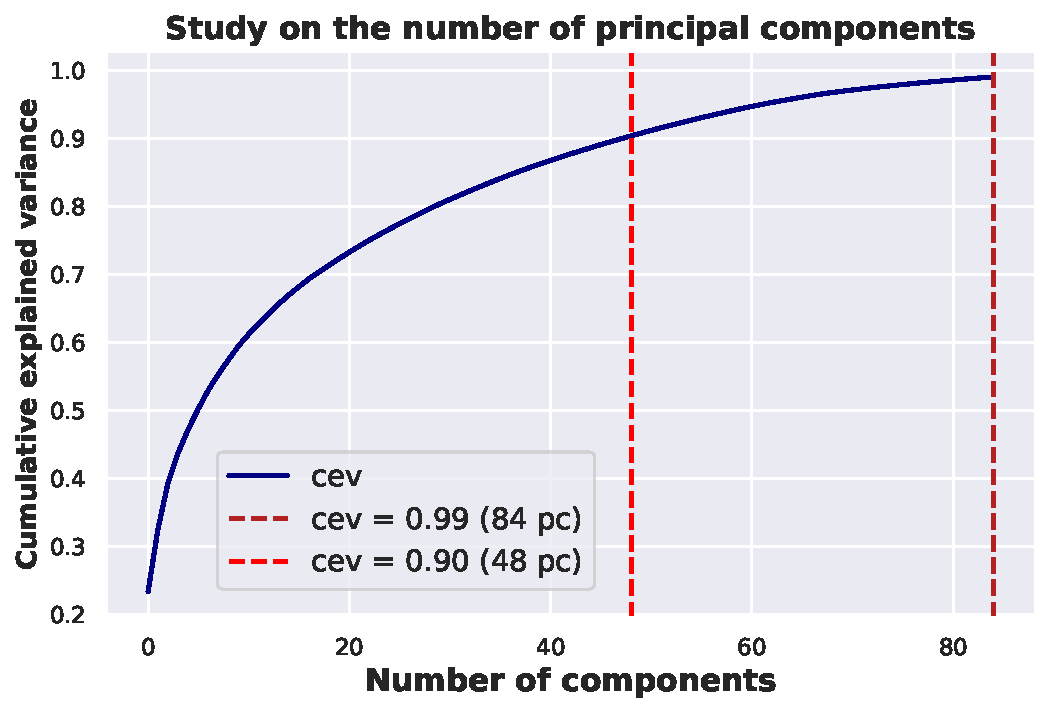
\includegraphics[width=0.4\textwidth]{pictures/cev.pdf}
	\caption{Cumulative explained variance ratio of the Principal Component Analysis applied to the features dataset.}
	\label{fig:cev}
\end{figure}
Looking at the line, one clearly see that, potentially, the 90\% of the information stored in the features can be reduced to just 48 values! The analysis presented in section \ref{sec:results} have been computed keeping, by default, the 99\% of the explained variance, i.e. 84 principal components. And the results are still quite nice. What would happen, instead, further reducing the number of eigenvalues to keep?
\begin{figure}[!h]
	\centering
	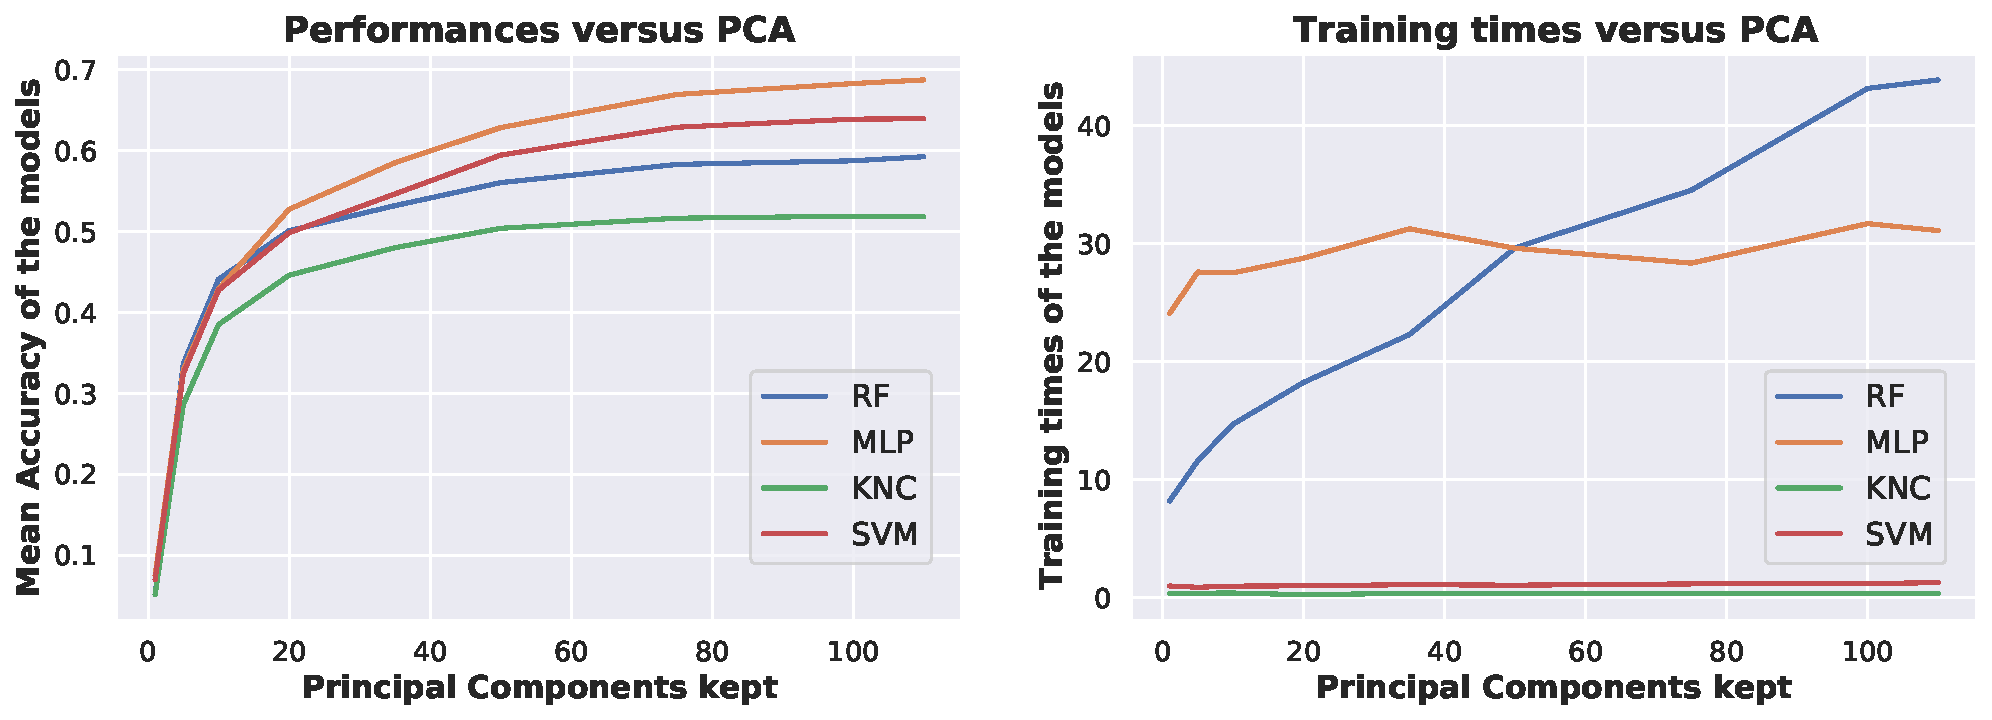
\includegraphics[width=0.5\textwidth]{pictures/pca_analysis.pdf}
	\caption{Comparison of mean accuracy reached and training times of the models for different numbers of principal components kept.}
	\label{fig:pca_analysis}
\end{figure}
The results shown in figure \ref{fig:pca_analysis} looks like exactly what we expected:
\begin{itemize}
	\itemsep0em
	\item in the left plot there are the mean accuracies obtained for the models trained: already after 40/50 principal components the lines start becoming flat, meaning that no significant further improvements are possible. And this is coherent with the explained variance ratio presented before (figure \ref{fig:cev}). Recalling section \ref{sec:features_extraction}, the vectors aimed to provide an high-level representation of the clips were created using an high number of features: probably so many (55) different quantities were unnecessary, and only half of them were sufficient. However, properly tuning the number of principal components, the problem vanishes.
	\item the right plot, instead, shows the computational times: the bigger are the input vectors, the larger will be the time necessary to make the classifier learn from them. With just 2000 clips the absolute difference is not so relevant, but the scaling behaviors of the lines, instead, are evident.
\end{itemize}


\subsubsection{Importance of the statistical estimators for the features distributions}
\label{app:stat_estimators}
In section \ref{sec:features_extraction} it has been explained that features distributions across frames were "summarized" using also their standard deviation, together with their mean, in order to properly represent also their irregularity and asymmetry. In figure \ref{fig:stat_estimators} it is shown the effective improvement, in term of accuracy, achieved training the four machine learning classifiers using just the mean or both the mean and the standard deviation.
\begin{figure}[!h]
	\centering
	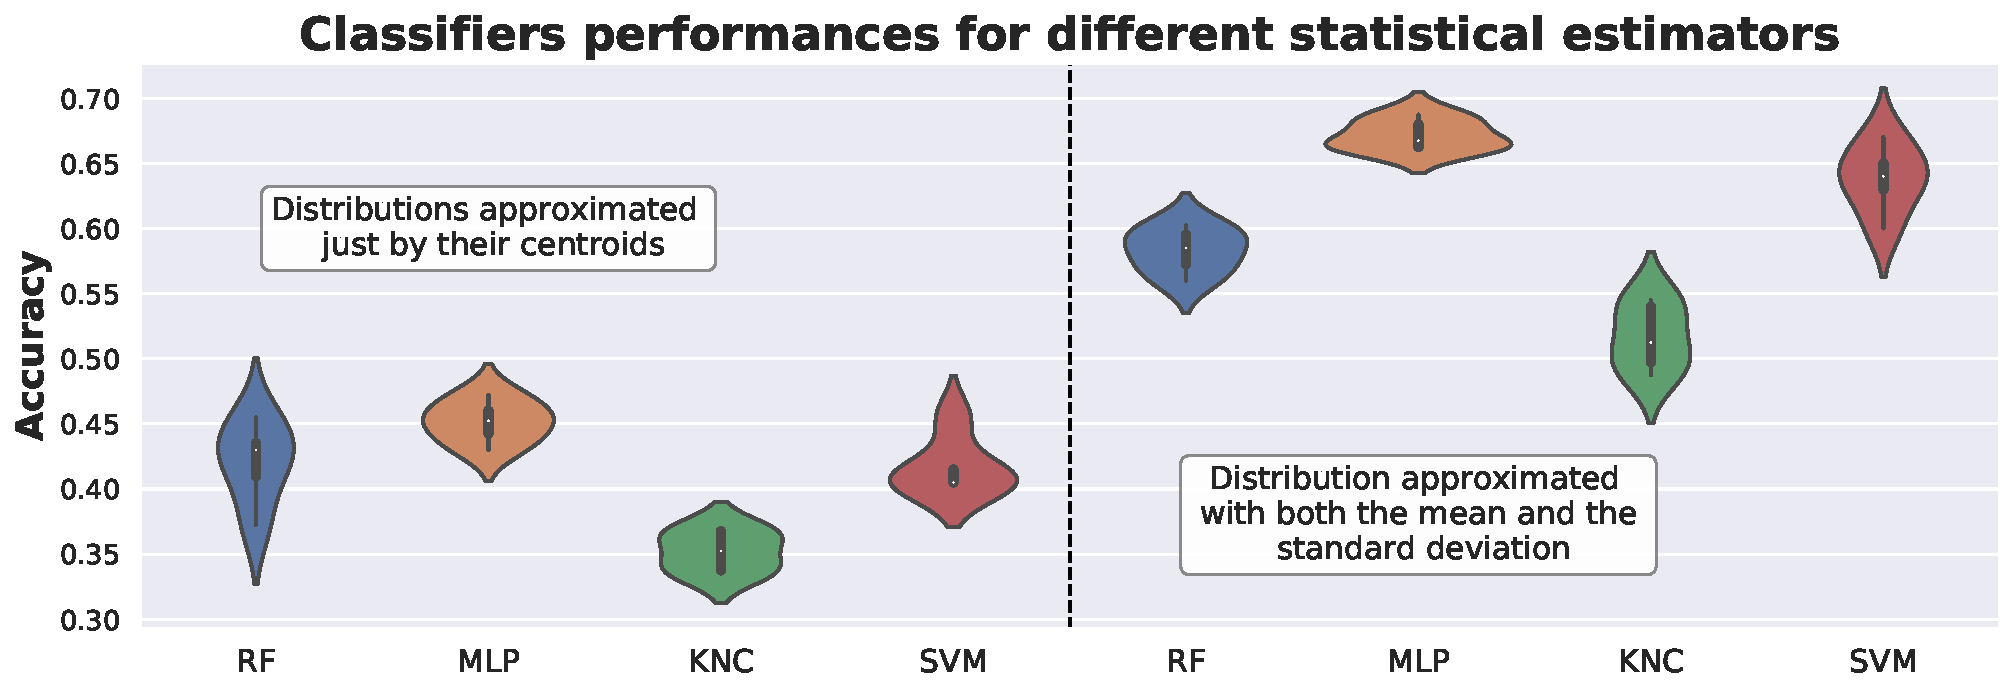
\includegraphics[width=0.47\textwidth]{pictures/stat_estimators.pdf}
	\caption{Comparison of the accuracy reached by the classifiers with one or two statistical estimators representing features distributions.}
	\label{fig:stat_estimators}
\end{figure}
The improvement is obvious: using both the mean and the standard deviation as statistics estimators provides almost a $+20\%$ to the accuracy obtained with all the models used. As expected, in fact, the distributions are, in general, quite asymmetric and non-gaussian, and taking just the average is probably an excess of reductionism.


\subsubsection{Importance of the silence removal step}
\label{app:importance_windowing}
The last step of the preprocessing phase explained in section \ref{sec:windowing} was the silence removal, i.e. the identification of fixed-size windows of zero energy, and their remotion from the successive calculations. In figure 	\ref{fig:silence_removal} are shown the differences, in term of accuracy, obtained with and without this windowing procedure.
`\begin{figure}[!t]
	\centering
	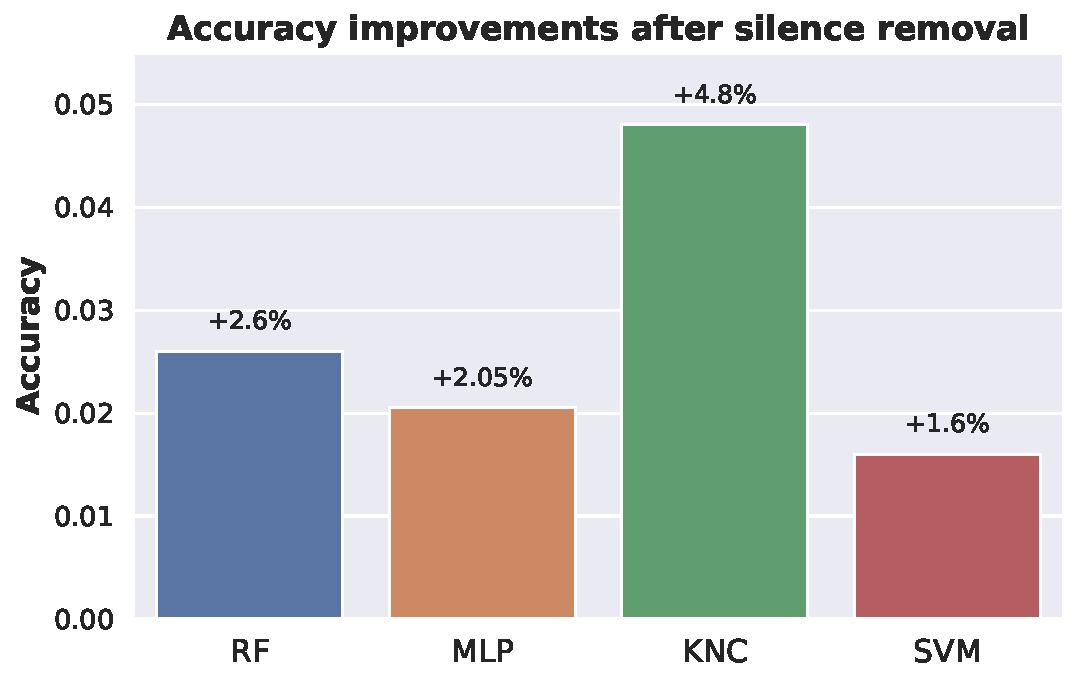
\includegraphics[width=0.47\textwidth]{pictures/silence_removal.pdf}
	\caption{Effective improvements in accuracy reached training the models with and without the silence removal phase.}
	\label{fig:silence_removal}
\end{figure}
And this is not even bad: getting a $+1\%/+5\%$ improvement in accuracy is nice, at the expenses of a small further preprocessing step.



\end{document}


